\documentclass[10pt,conference,compsocconf]{IEEEtran}

%Deadline: April 8, 2015
%Call for papers: http://www.computer.org/web/computingnow/swcfp6

\usepackage{url}
\usepackage[table,xcdraw]{xcolor}
\usepackage{eurosym}
\usepackage{amsfonts}
\usepackage{balance}
\usepackage{cite} %this package is awesome - it reorders lists of citations to be in numeric order
\usepackage{pifont}
\usepackage{eqparbox}

% Tables
\usepackage{booktabs}
\usepackage{pbox}
\renewcommand{\arraystretch}{1.2} 
\usepackage{arydshln}
%\renewcommand*\cmidrule{} % No middle lines
%\renewcommand{\arraystretch}{1.5} % Additional spacing with no middle lines
%\renewcommand*\cmidrule{\hdashline[1pt/2pt]}% Dashed middle lines
\renewcommand*\cmidrule{\midrule[0.001em]} % Thin middle lines
%\renewcommand*\cmidrule{\midrule} % Thick middle lines

%Images
\usepackage[pdftex]{graphicx}
\graphicspath{ {}{img/} }
\DeclareGraphicsExtensions{.pdf,.jpg,.png}

\hyphenation{second-ly ap-pen-dix}

\clubpenalty = 10000
\widowpenalty = 10000
\displaywidowpenalty = 10000

\newcommand{\todo}[1]{\textbf{TODO: #1}}
\newcommand{\ignore}[1]{}

\begin{document}
\bstctlcite{IEEEexample:BSTcontrol}
%
% paper title
% can use linebreaks \\ within to get better formatting as desired
\title{Smell Detection and Refactoring in End-User Programming Languages}
%\title{Perspectives on End-User Refactoring: Past, Present, and Future}

\author{\IEEEauthorblockN{Felienne Hermans, David Hoepelman}
\IEEEauthorblockA{Delft University of Technology\\
Mekelweg 4\\
2628 CD Delft, the Netherlands\\
f.f.j.hermans@tudelft.nl}


\and
\IEEEauthorblockN{Kathryn T. Stolee}
\IEEEauthorblockA{Iowa State University\\
209 Atanasoff Hall\\
Ames, IA 50011-1041\\
kstolee@iastate.edu}
}

\maketitle


\begin{abstract}
In the workforce today, millions of people program without degrees or professional training in software development. 
These end-user programmers write code to design hardware circuits, combine web information, and impact business decisions. 
Software engineering research into refactoring has traditionally focused on professionally used object-oriented programming languages, 
yet other domains and languages also suffer from code smells in need of refactoring. 

In this work, we explore recent research in three end-user domains and languages, spreadsheets in Microsoft Excel, web mashups in Yahoo!\ Pipes, and system design in National Instruments' LabVIEW. 
Through exploring the commonalities and differences among the domains, we
1)~show how these end-user domains benefit from prior research on refactoring object-oriented languages,
2)~discuss unique smell detection and refactoring opportunities for these domains and how they can translate to professional languages, and
3)~identify future opportunities for smell and refactoring research in these studied domains as well as other end-user programming domains. 
\end{abstract}


\begin{IEEEkeywords}
code smells;
end-user programming;
refactoring;
\end{IEEEkeywords}

\section{Introduction}
End-user programmers are said to outnumber the amount of professional programmers three times over \cite{Scaf2005}.
These end-user programmers perform a wide variety of tasks within their organizations, ranging from building or maintaining applications to simple data manipulation in a spreadsheet.
While performing these tasks, end-user programmers face many of the challenges of professional developers, such as identifying faults, debugging, or understanding code written by someone else~\cite{Ko2011}.
Similar to code written by professional developers, end-user artifacts may have a long life-span, the average lifespan of a corporate spreadsheet being five years~\cite{Hermans2011}.
During this long lifespan, end-user artifacts are modified, often by different people.
These properties make them, like source code artifacts, vulnerable to \emph{smells}. 

Smells in end-user programming have been a topic of research over the past few years. Most notable are structural smells in Yahoo!\ Pipes web mashups~\cite{Stolee2011} and  Excel spreadsheets \cite{Hermans2012inter} and performance smells in LabVIEW code \cite{chambers2013smell}.
Experiments in all these areas have shown that end-user programmers understand smells and often prefer versions of their code that are non-smelly \cite{Hermans2012intra, StoleeTSE2013, chambers2013smell}.
Alleviating those smells can be achieved with refactoring.

Refactoring was first introduced as a systematic way to restructure source code and facilitate software evolution and maintenance. Martin Fowler later introduced the concept of code smells \cite{Fowl1999}. 
Refactoring code is often motivated by noticing a code smell, which signals the opportunity for improvement.

The taxonomy of smells outlined in Fowler's text pertained mostly to object-oriented code, and professional programming languages were the focus for at least the first decade of refactoring and code smell research~\cite{Mens:2004:SSR:972215.972286}.
Since 2011, however, refactoring and smell definitions have been adapted and extended to other 
programming language paradigms, including web mashups~\cite{Stolee2011, StoleeTSE2013}, Excel spreadsheets~\cite{Hermans2011, Hermans2012inter, hermans2014bumblebee}, and LabVIEW programs~\cite{chambers2013smell}, all of which are end-user programming domains. 

Considering the large number of end-user programmers, the longevity of their artifacts, and the impact of smells on understandability, errors, and performance, supporting end-user programmers in code smell detection and refactoring is valuable.
The applicability of smells, originally created to detect weaknesses in source code, to other domains shows how powerful the concept is. Furthermore, studying the smells and refactorings in a fresh context provides new insight on how to use smells in software engineering and  even suggests new types of smells. This is what we study in this paper.
The contributions of this work are:

\begin{itemize}
%	\item Synthesis of recent research in smell detection and refacotring for end-user programming languages
%	\item Motivation for the study of smells and refactoring for end-user programming languages based on empirical evidence
	\item Synthesis and catalog of object-oriented-inspired code smells  and refactoring in end-user programs
	\item Discussion of how smells and refactoring in  end-user domains may translate to professional languages
	\item Identification of future opportunities for smell detection and refactoring in end-user programming domains
\end{itemize}


\section{Background}
\label{sec:background}

Here, we briefly explore each end user domain before presenting the relevant code smells in  Section~\ref{sec:smells} and refactorings in Section~\ref{sec:refactoring}.

\paragraph{Excel}

\begin{figure}
\caption{Microsoft Excel 2013 showing a spreadsheet}
\centering
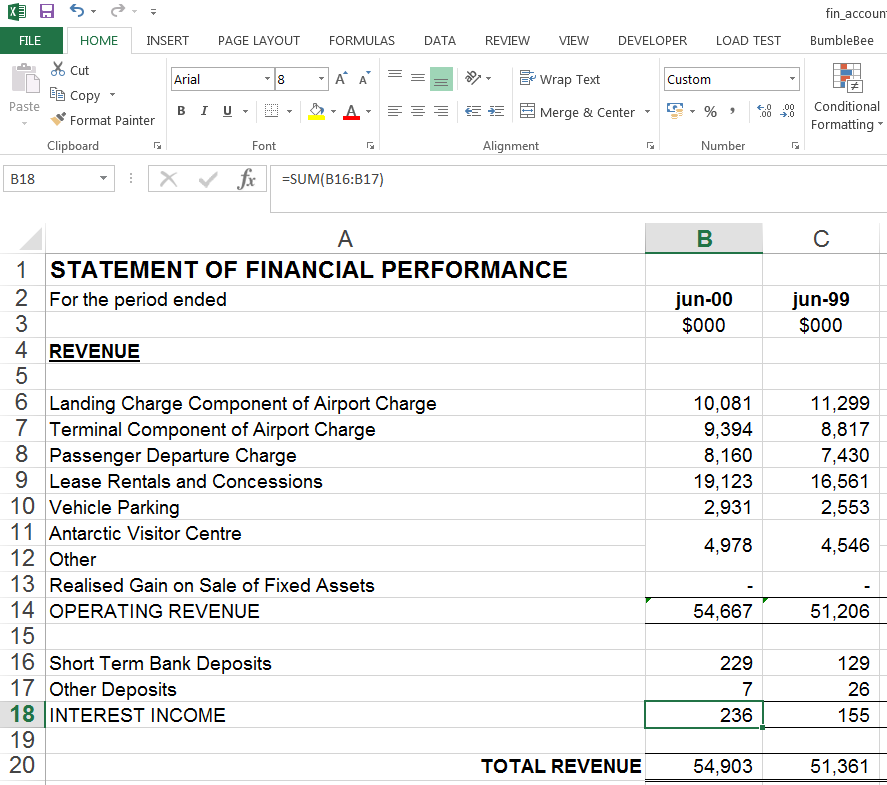
\includegraphics[width=\columnwidth]{excel-2}
\label{fig:spreadsheetexample}
\end{figure}

Spreadsheets are very commonly used in businesses, from inventory administration to educational applications and from scientific modeling to financial systems.
Winston ~\cite{Wins2001} estimates that 90\% of all analysts in industry perform calculations in spreadsheets. 
Microsoft Excel is by far the most used, and therefore most studied, spreadsheet program, but other implementations exists and are similar.

In modern spreadsheet programs, a \textit{cell} can contain a single \textit{formula} which performs a calculation, and a table of cells is bundled in a \textit{worksheet}.
A \textit{workbook} consist of a collection of worksheets.
Formulas can reference other cells in the same or in different workbooks and worksheets.


\paragraph{Yahoo!\ Pipes}
A web mashup is a program that collects and combines information from various
sources. 
In  Yahoo!\ Pipes, the information comes from RSS feeds. Figure~\ref{fig:ypexample} shows an example Yahoo!\ Pipes program. The boxes represent modules connected by wires. 
Abstraction is possible with \emph{subpipe} modules, which allow a programmer to insert a different pipe as a subroutine, appearing like a standard module. 

\begin{figure}
\caption{Example of a program in Yahoo!\ Pipes. It has five RSS feed data sources, each in a \emph{Fetch Feed} module, feeding to a \emph{Union} module that concatenates the feeds, a \emph{Truncate} module that limits the number of items to 15 prior to the final \emph{Pipe Output}. }
\centering
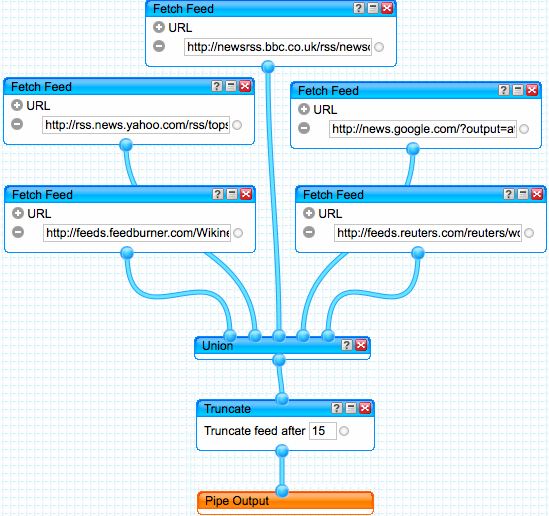
\includegraphics[width=\columnwidth]{yp-1}
\label{fig:ypexample}
\end{figure}


\paragraph{LabVIEW}
\begin{figure}
\caption{Example of a G program from the LabVIEW manual. This program takes samples from sensors and show their Time Domain Sequence and DC-Centered Spectrum.}
\centering
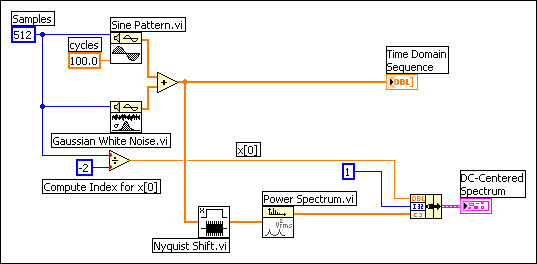
\includegraphics[width=\columnwidth]{labview-1}
\label{fig:labviewexample}
\end{figure}

LabVIEW is a hardware system design environment that features the visual programming language ``G'' as one of its primary features.
An example of a G program can be found in Figure \ref{fig:labviewexample}.
G is a dataflow language which means a program is represented as a directed graph where data ``flows'' between nodes through their edges.
As such the two most important primitives in G are the edges called \textit{wires} and nodes called \textit{virtual instruments}.
VI's are very similar to functions, because they perform an operation on inputs and provide outputs.
Wires with no source VI are inputs and wires without a destination VI are outputs. 


\section{Smells in end-user programs}
\label{sec:smells}
Research into end-user programming smells has had two approaches, which are not mutually exclusive.
The first approach is to take existing smells for OO programming languages, usually those defined by Fowler~\cite{Fowl1999}, and transform them to be applicable to the end-user environment \cite{Hermans2012inter,Hermans2012intra,Stolee2011,StoleeTSE2013, chambers2013smell}.
The second approach is to define smells tailored to the end-user environment.
This can be done by interviewing experienced end-users to see which smells they perceive \cite{chambers2013smell}, by looking at user reports like forum or newsgroup posts~ \cite{badame2012refactoring,chambers2013smell}, or by analyzing publicly available artifacts \cite{Stolee2011,StoleeTSE2013}.

This section provides an overview of different smells that researchers have found to be applicable to end-user artifacts using both the above described approaches and proposes future directions for smell detection in these domains. 

\begin{table*}
\caption{Code Smells in End-User Programs
\label{table:oosmellslarge}}
\centering
\sffamily
\begin{tabular} {@{}llll@{}}
\toprule
\textbf{OO Smell}
	& \textbf{Excel}
	& \textbf{Yahoo!\ Pipes}
	& \textbf{LabVIEW}
\\ \midrule
Feature Envy
	& Feature Envy \cite{Hermans2012inter}
	& Feature Envy *
	& ~~ 
\\ \cmidrule
Long Method
	& Multiple operations \cite{Hermans2012intra}
	& Long Module*
	& Large Virtual Instrument *
\\ \cmidrule
Message Chain
	& Long Calculation Chain \cite{Hermans2012intra}
	& 
	& 
\\ \cmidrule
Inappropriate Intimacy
	& Inappropriate Intimacy \cite{Hermans2012inter}
	& Inappropriate Intimacy *
	& ~~ 
\\ \cmidrule
Lazy class or Middle Man
	& Middle Man \cite{Hermans2012inter}
	& Unnecessary Abstraction \cite{StoleeTSE2013}
	& ~~ 
\\ \cmidrule
Many Parameters
	& Multiple References \cite{Hermans2012intra}
	& 
	& Many Control Terminals *
\\ \cmidrule
Duplicate Code
	& Duplicated Formulas \cite{Hermans2012intra}
	& Duplicate Modules, Duplicate String or
	& Isomorphic Path *
\\ % Continuation
& 
& Isomorphic Path \cite{StoleeTSE2013}
& 
\\ \cmidrule
Dead Code
	& ~\ding{55}
	& Disconnected or Dangling Modules \cite{StoleeTSE2013}
	& Disconnected or Dangling Elements *
\\ \cmidrule
Unused Field
	& ~\ding{55}
	& Noisy Module \cite{StoleeTSE2013}
	&
\\ \cmidrule
No-op
	& Redundant Operations *
	& Unnecessary Module \cite{StoleeTSE2013}
	& Redundant Operations \cite{chambers2013smell}
\\ \cmidrule
Use of Deprecated Interfaces
	& Deprecated Functions *
	& Deprecated Module or Invalid Source \cite{StoleeTSE2013}
	&
\\ \bottomrule
\multicolumn{4}{c}{} \\
\multicolumn{4}{l}{\ding{55} : Not applicable due to the nature of the paradigm} \\
\multicolumn{4}{l}{* : Proposed name, likely future opportunity not supported by prior work}\\
\multicolumn{4}{l}{$\langle$blank$\rangle$ : Not discussed in this work, possible future opportunity} \\
\end{tabular}
\end{table*}

\subsection{OO Smells in End-User Programs}
\label{sec:smells:oo}
 We summarize the OO smells present in the three end-user languages, Excel spreadsheets, Yahoo!\ Pipes mashups, and LabVIEW designs, in Table~\ref{table:oosmellslarge}.
 
 Overall, we observe a lot of similarities in the code smells studied. For example, the \emph{Duplicate Code} and \emph{Many Parameters} smells have been studied in all three languages. Some smells, like the \emph{Long Method} smell, have been studied in only one domain but are likely applicable in other domains, too (marked with *). These smells present opportunities for future research (see Section~\ref{subsec:futuresmells}).
 
% A small number of smells are definitely not applicable (\ding{55}) because of differences in the domains. Spreadsheets, for example, cannot contain dead code because the user might still be interested in a piece of data even if it is not used anywhere else in the spreadsheet.

 \subsubsection{Excel}
Hermans et al. \cite{Hermans2012inter,Hermans2012intra} analogize a workbook to a program, a worksheet to a class inside that program and a cell to a method and use this to transform nine of Fowlers smells.
An example of this is the \emph{Long Method} smells, which translated the \emph{Multiple Operations} smells because formulas with a lot of operations are long and suffer from similar problems as long methods.

\subsubsection{Yahoo!\ Pipes}
Stolee and Elbaum~\cite{Stolee2011, StoleeTSE2013} treat a Yahoo!\ Pipes mashup as a class and each module as a method.  Fields in a module are treated as parameters. Using this analogy,  several OO smells were mapped to this language. The most common smell, appearing in nearly one-third of the 8,000 pipes studied, was \emph{Duplicate Strings}, an instance of Fowler's \emph{Duplicate Code} smell. 
\emph{Duplicate Modules}, impacted nearly one-quarter of the pipes studied. 
 Overall, 81\% of the programs studied from the Yahoo!\ Pipes community had at least one smell. 
 
Yahoo can deprecrate modules and not replacing them has similar problems to using deprecated or old versions of interfaces, which is the reason for the \emph{Deprecated Module} smell.

\subsubsection{LabVIEW}

Current work on LabVIEW smells has been focused on smells with potential permance impacts.
As most OO smells do not have a direct impact on performance, the equivalents of OO smels for LabVIEW have not yet been defined.

\subsection{Domain-Specific Smells}
\label{sec:smells:domain}
The end-user programming environments offer many opportunities to define smells based on user behavior or unique elements of the domain. For example, access to large repositories of programs can lead to smells that deviate from best practices in programming. In this section, we explore opportunities for new smells in end-user domains that extend beyond the OO-inspired smells described in Section~\ref{sec:smells:oo}. 

\subsubsection{Excel}

In spreadsheets data is often processed by having each record in a row and having a column with identical formulas to perform some calculation.
This leads to the definition of the \emph{Inconsistent Formula} smell, which occurs if a single, or small number, of cells contain a different formula while its neighbors or other cells in the row or column contain an identical formula.
Interestingly this smell is already detected by Microsoft Excel which warns the user about it.

Another smell specific to spreadsheets is when a formula references an empty cell, which is often in error \cite{cunha2012towards}.
This is comparable to a null pointer in a program, but because a spreadsheet contains both the input data and logic we can mark it as a smell.

\subsubsection{Yahoo!\ Pipes}
%Talk about smells unique to the domain
By exploring a large subset of the Yahoo!\ Pipes repository, Stolee and Elbaum identified two smells based on the presence of broken data sources and the use of deprecated modules~\cite{StoleeTSE2013}.
A reference to a broken data sources  is similar to opening a non-existing file.
In Java, this would manifest as an error with a {\tt FileNotFound} exception at runtime.
Such exceptions are not in the Yahoo!\ Pipes language, which is th reason to mark it as a smell. 
%Talk about deriving smells from the community
Similar exploration was used to  identify common programming practices, marking deviations from those practices as smells. 
This is similar to identifying  smells  as anti-patterns  and could be extended to any language. 


\subsubsection{LabVIEW}

G programs are often run in an embedded or real-time environment, and as such are very susceptible to performance problems. This motivated Chambers and Scaffidi \cite{chambers2013smell} to G smells with potential performance implications and implement heuristics to identify these smells.
An example of this is the ``\textit{Sequence instead of State machine}'' smell which is a smell because the G compiler can better optimize state machines.

Because G program heavily rely on concurrency it is susceptible to problems which can cause problems in concurrent programs such as non-reentrant VI's.

\subsection{Future Opportunities for Smell Detection}
\label{subsec:futuresmells}
There are several OO code smells in Table~\ref{fig:ypexample} that apply to all three domains, such as \emph{Duplicate Code}. However, there are other smells that could apply to additional domains, but have not been studied in prior work. Here, we discuss the potential of generalizing some of the OO and domain-specific smell definitions to additional domains. 

\subsubsection{Excel}
Most of the smells studied in other end-user domains have been studied in Excel spreadsheets, but there is some future potential on the areas of redundancy and deprecation.

Currently all work has focused on Microsoft Excel.
However, other spreadsheet software exists and operates on the same principles.
Thus there is an opportunity to confirm that the identified smells apply in other spreadsheet software.

\subsubsection{Yahoo!\ Pipes}
\label{sec:smells:future:yp}
%Many of the smells studied in Excel and LabVIEW could apply to Yahoo!\ Pipes, and in particular, \emph{Feature Envy} and \emph{Inappropriate Intimacy}. 
%uses methods of another class excessively - envy
The \emph{Feature Envy} smell could also apply when introducing abstraction. For example, if a pipe has several instances of the same subpipe module, this could be excessive use of another class. 

%depends on implementation of another class too much - intimacy
When a program uses too much abstraction relative to the size of the pipe, it could suffer from \emph{Inappropriate Intimacy} by depending too much on the implementation of the other class. In fact, in an empirical evaluation, programmers often preferred pipes without subpipe modules because they were easier to understand~\cite{StoleeTSE2013}. 

%long method
A \emph{Long module} smell could apply when a module has a large number of fields. For example, the \emph{Fetch Feed} module, as in Figure~\ref{fig:ypexample}, can hold one or more URLs. When the number of URLs makes the method so big it does not fit on the screen, this would likely impact the understandability of the pipe. 

Drawing inspiration from the domain-specific \emph{Inconsistent Formula} smell in Excel, identifying program patterns that are close, but not exactly the same, could identify missed opportunities for abstraction or errors in the mashup structure. 

\subsubsection{LabVIEW}

Research into smells for LabVIEW has focused mostly on performance problems, while traditionally research into code smells and refactorings has focused on maintainability and code quality.

As such inspiration could be drawn for smells that do not necessarily have an impact on performance.
We have defined some OO smells that have parallels in LabVIEW.

A \emph{Large Virtual Instrument} would have similar problems to a \emph{Long Method} and could be divided, and like \emph{Many Parameters} make a method hard to understand \emph{Many Control Terminals} could increase the difficulty of understanding a VI.
If a block diagram contains a combination of nodes wired identically multiple times, they are \emph{Duplicated Nodes} and should be extracted into their own VI. 

\begin{table*}
\caption{Code Refactorings in End-User Development}
\label{table:ooreflarge}
\centering
\sffamily
\begin{tabular} {@{}llll@{}}
\toprule
\textbf{OO Refactoring}
	& \textbf{Excel}
	& \textbf{Yahoo!\ Pipes}
	& \textbf{LabVIEW}
\\ \midrule
Remove Parameter
	& Move References \cite{Hermans2012intraExt}
	& Clean Up Module \cite{StoleeTSE2013} 
	& Remove Terminal \cite{chambers2015impact}
\\ \cmidrule
Extract Method
	& Extract Subformula \cite{Hermans2012intraExt,badame2012refactoring}
	& Extract Local Subpipe \cite{StoleeTSE2013}
	& Extract Virtual Instrument \cite{sui2008automated}
\\ \cmidrule
Inline Method
	& Inline Formula *
	& Push Down Module \cite{StoleeTSE2013}
	& Inline Virtual Instrument *
\\ \cmidrule
Substitute Algorithm
	& Replace Formula *
	&  \pbox{4.5cm}{Merge Redundant Modules or Colapse Duplicate Path\cite{StoleeTSE2013} }
	& Substitute Block Diagram *
\\  \cmidrule
Library Migration~\cite{Balaban:2005:RSC:1103845.1094832}
	& Migrate Formulas \cite{hermans2014bumblebee}
	& Replace Deprecated Modules \cite{StoleeTSE2013}
	& 
\\  \cmidrule
Define named constant
	& Extract Literal \cite{badame2012refactoring}
	& Pull Up Module \cite{StoleeTSE2013}
	& ~~
\\ \cmidrule
Remove dead code
	& \ding{55}
	& \pbox{4.5cm}{Remove  Disconnected or Dangling Modules \cite{StoleeTSE2013}}
	& \pbox{4.5cm}{Remove Disconnected or Dangling Elements *}
\\ \cmidrule
Remove No-op
	& Remove Redundant Operations *
	& Remove Lazy Module \cite{StoleeTSE2013}
	& Remove Redundant Operations \cite{chambers2015impact} \\
\bottomrule
\multicolumn{4}{c}{} \\
\multicolumn{4}{l}{\ding{55} : Not applicable due to the nature of the paradigm} \\
\multicolumn{4}{l}{* : Proposed name, future opportunity not supported by prior work.}\\
\multicolumn{4}{l}{$\langle$blank$\rangle$ : Possible future opportunity, not discussed in this work}
\end{tabular}
\end{table*}


\section{Refactoring end-user programs}
\label{sec:refactoring}

A way to solve smells is by refactoring, changing an artifact so that it no longer contains the smell without changing its behavior or output.
As with the smells, many refactorings are inspired by the OO domain, while others are specific to the end-user domain. 

\subsection{OO Refactorings}
Table~\ref{table:ooreflarge} lists the OO refactorings adapted for the end-user domains, identifying those that have been studied and likely apply.
Some of these come from Fowler's definitions while others are from past refactoring research. 

\subsubsection{Excel}

Hermans et al. \cite{Hermans2012intraExt} define refactorings corresponding to most of their smells, but most do not have a direct OO equivalent.
One that was defined earlier by Badame and Dig \cite{badame2012refactoring} is the direct equivalent of \emph{Extract method} and is called \emph{Extract Row or Column} by Badame and \emph{Extra subformula} by Hermans.
Because Hermans equates formulas to methods, refactorings that change the parameters of a method also have a direct equivalent in spreadsheet by changing the references in a formula. For example \emph{Remove Parameter} becomes \emph{Remove reference}.
 
\subsubsection{Yahoo!\ Pipes}
The refactorings studied in Yahoo!\ Pipes aim to make pipes smaller, less complex, more maintainable, and easier to understand~\cite{StoleeTSE2013}.
Some of the refactorings translated easily from the OO domain. For example, removing dead code was as simple as \emph{removing disconnected, dangling, or swaying modules} or removing parameters in \emph{clean up module}~\cite{StoleeTSE2013}.
The \emph{Extract Local Subpipe} refactoring involved extracting a connected set of modules into into a subpipe and thus is identical to the \emph{Extract Method} refactoring.
Once the subpipe was created, all  parts of the program with the same pattern of connected modules were replaced with the subpipe module. 

\subsubsection{LabVIEW}

While Chambers and Scaffidi have done some work on refactoring \cite{chambers2015impact}, few of their refactorings have a direct OO equivalent. \emph{Remove Redundant Operation} maps to G as removing a No-op.
However, Sui et. al \cite{sui2008automated} have done some work on refactoring general visual dataflow languages and defined some refactorings which are applicable to G.
Most notably their work defines the \textit{Extract Virtual Instrument} when applied to G.

\subsection{Domain-Specific Refactorings}

Building off the discussion of domain-specific smells in Section~\ref{sec:smells:domain}, here we discuss opportunities for domain-specific refactorings. 

\subsubsection{Excel}

Some work has been done on refactoring formulas inside a single cell of a spreadsheet. Badame and Dig \cite{badame2012refactoring} define the \textit{Guard Call} refactoring, which places a conditional check around a (sub)formula that can return an error, for example a check for a division by zero.

Hermans and Dig \cite{hermans2014bumblebee} have followed up on this and define a generalized way to transform formulas into other formulas, in a way that is very similar to how a regular expression or patterns works in some modern programming languages.

\subsubsection{Yahoo!\ Pipes}
\label{sec:yp:domainrefactor}
%Opportunities for domain-specific refactorings stem from the domain-specific code smells. 
%For example, b
When a program used a syntax that was different from the community standard, as detected by the \emph{Non-conforming Module Orderings} smell, the \emph{Normalize Order of Operations} refactoring could be applied to change this. The end-user programmers preferred the standardized version \cite{StoleeTSE2013}. Another refactoring replaces the usage of deprecated modules.

\subsubsection{LabVIEW}

Chambers and Scaffidi \cite{chambers2015impact} have defined transformations for most of their performance smells, but not all are refactorings because most change the program behavior.
However, some refactorings which only slightly change program behavior were effective. For example introducing a 1ms pause inside a loop without a pause decreased execution time by 37\%.

\subsection{Future Opportunities for Refactoring}

Future opportunities for refactoring research are abound in these domains. We will discuss a few of these.

\subsubsection{Excel}

While some work has been done on refactoring the structure of the whole spreadsheet instead of only formulas in cells, there is an opportunity for more research. 
Specifically how worksheets and regions of cells are similar and different to classes and methods can be further explored to define refactorings.
A refactoring which was not previously defined is the \emph{Inline Formula} refactoring, which is done by replacing the reference to a cell by its formula and deleting the original cell, although this might not be possible if the cell is referenced as part of a range.
The \emph{Remove Redundant Operations} refactoring could be adapted from other domains and is defined as removing parts of a formula which do not impact the result.

%Another domain to draw inspiration from is (relational) databases.
%As spreadsheets are often used to store data and lookup functions are similar to the \texttt{JOIN} functionality in SQL, spreadsheets might benefit from knowledge gained in database theory, for example normalization.

Inspiration might also be drawn from refactoring in dataflow languages like Yahoo! Pipes and LabVIEW G, because a spreadsheet can also be represented as a dataflow program in which cells are nodes and reference to cells are wires.

\subsubsection{Yahoo!\ Pipes}
Handling the smells identified in future work in Section~\ref{sec:smells:future:yp} involves small modifications on existing refactorings or new refactorings. For a small modification, the \emph{Long Module} smell can be addressed with \emph{Extract Local Subpipe}. 
Addressing \emph{Feature Envy} may be possible in some cases by using \emph{Collapse Duplicate Path} when the subpipes are connected to modules that form similar paths in the pipe.
With \emph{Inappropriate Intimacy}, a new refactoring should be introduced that is the reverse of \emph{Extract Local Subpipe}, which would inline the subpipe logic. 
 %However, in the general case, refactoring this smell may not be feasible. 

% Removed this because it is already slightly adressed in Domain-specific refactorings - David
%In a qualitative analysis of the end-user preferences for Yahoo!\ Pipes programs, the participant responses showed preference toward programs with familiar elements~\cite{Stolee2015}. This opens an opportunity and perhaps a need to define code smells and refactorings based on end-user experience. 

\subsubsection{LabVIEW}

Similarly to the research into smells in LabVIEW G programs, research into refactoring of G programs has also been driven by the desire for performance improvements. Refactorings which do not directly impact performance have only been theoretically explored for general dataflow languages \cite{sui2008automated}.

\section{Related Work}
\label{sec:related_work}

This paper builds upon the extensive body of work related to code smells and refactoring. For an extensive overview we review the reader to the work of Mens and Tourw\'{e} \cite{mens2004survey}.

%\subsection{Smells based on user input}
%\label{subsec:related_datasmells}
In end-user programming environments user input and logic are often more closely linked than they are in general purpose languages.
As such analyzing the input data as opposed to the logic can also be used to detect problems.

Cunha et. al \cite{cunha2012towards} claim to define code smells for spreadsheet, but for most of their smells they look at different types of anomalies in the data of a spreadsheet and define these as smells.
%Examples of this are \textit{Standard Deviation} which occurs if one assumes a normal distribution for a column in numeric values and the column contains values which fall outside two standard deviations.
In more recent work, Barowy et. Al \cite{barowy2014checkcell} take a very similar but more formalized approach which they label ``Data Debugging''.
Their solution uses statistical analysis to find values with an unusually high impact on the calculated results in a spreadsheet, as such values are likely either very important or erroneous.

\section{Discussion}
\label{sec:discussion}

Based on the research and results for smell detection and refactoring in end-user programming domains, there are many directions for future work in the domains studied and other end-user domains.

\subsection{Future Opportunities in Other EUP Domains}
End-user programming domains extend beyond spreadsheets, web mashups, and system designs. Stolee and Elbaum explore future opportunities for refactoring in educational programming languages~\cite{StoleeTSE2013}. Additional opportunities in educational languages exist in LEGO Mindstorms, which is based off the G language for LabVIEW.  Another end-user programming domain that could benefit from smell analysis and refactoring is mathematics languages. These include MATLAB, Sage, or Mathematica.

In particular, the smells related to duplication and poor construction (e.g., long method, many parameters, dead code) are  prevalent in the three domains studied. These smells -- and their respective refactorings -- likely exist in other end-user programming domains, and likely hinder the understandability and maintainability of those programs. Worse even, these smells likely also lead to errors, and thus are worthy of our attention. 


%\subsection{Future Opportunities in Professional Languages}
%In end-user programming languages, it has been shown that code smells impact the understandability of
%source code~\cite{StoleeTSE2013}. Additionally, being presented with code smells can motivate end-user programmers to improve their code~\cite{chambers2013smell}, and smells in spreadsheets have even been known to reveal actual errors~\cite{Hermans2012intra}. These lessons could extend to professional programming languages. but further study is needed. 
% outside of the end-user programming domains. 
%There has been successful in using automating smell detection, for example, during agile development (e.g.,~\cite{Schumacher:2010:BES:1852786.1852797}). Paired with the end-user evidence, a stronger case can be made to integrate automated smell detection in many domains. 

%\todo{Other data flow languages could benefit from \emph{normalize order of operations} to improve understandability (as it does with YP). }

\subsection{Threats to Validity}
The threats to validity of this work inherit the threats to validity of the original studies~\cite{Stolee2015, Stolee2011, StoleeTSE2013, Hermans2011, Hermans2012intra, Hermans2012inter, hermans2014bumblebee, chambers2013smell, chambers2015impact, badame2012refactoring}. In addition, we note that the authors of this work have pioneered smell detection and refactoring research in spreadsheets and Yahoo!\ Pipes, but are not involved with LabVIEW. Thus, the opportunities for future work in this area may not be complete.  

\section{Concluding Remarks}
\label{sec:conclusions}
This paper presents an overview of the work in smell detection and refactoring for end-user programming languages. More specifically, it synthesizes work on Yahoo! Pipes, Excel and LabView. We explore commonalities between these works and identify opportunities for application of methods from these domains to others and to generic programming languages. As we move forward, we see many opportunities to explore additional smells and refactorings in the domains studied, in other end-user programming domains, and even in extending the findings to professional languages. 

\balance

% Work that wasn't directly referenced but should still appear in the literature list
\section*{Acknowledgements}
This work is supported in part by  NSF SHF-EAGER-1446932 and the Harpole-Pentair endowment at Iowa State University. \todo{Felienne - do you have funding agencies to thank?}


\bibliographystyle{IEEEtran}
\bibliography{literaturelist}

\end{document}


